\documentclass[UTF8]{ctexart}
\usepackage[a4paper, top = 3cm, bottom = 3cm, left = 2cm, right = 2cm]{geometry}
\usepackage{graphicx}
\usepackage{fancyhdr}
\pagestyle{plain}   % 使用plain样式，页码在页脚居中
\usepackage{amsmath}
\usepackage{float}
\usepackage{xcolor}

\usepackage{caption}
\captionsetup[figure]{labelformat = empty}

\usepackage{enumitem}
\setlist[enumerate]{label=(\arabic*)}   % 标号默认为(1)(2)(3)

\newcommand{\rs}{\text{ rad/s}}
\newcommand{\wc}{\omega_\text{c}}
\newcommand{\ex}[1]{\text{e}^{#1}}

\begin{document}

\section*{2025-2026学年秋学期《控制工程基础》期末回忆卷}

\begin{center}
    折一只纸鹭
\end{center}

\subsection*{第一题（15分）}

如图所示的机械系统，$m_1,m_2$ 为物块质量，$k$ 为弹簧的弹性刚度，$\mu$ 为阻尼器的黏性阻尼系数. 输入为力 $f_\text{i}(t)$，输出为位移 $x_\text{o}(t)$. 忽略质量块与地面之间的摩擦.

\begin{enumerate}
    \item 列出系统的微分方程.
    \item 画出系统的方块图.
    \item 求系统的传递函数.
\end{enumerate}

\begin{figure}[H]
    \centering
    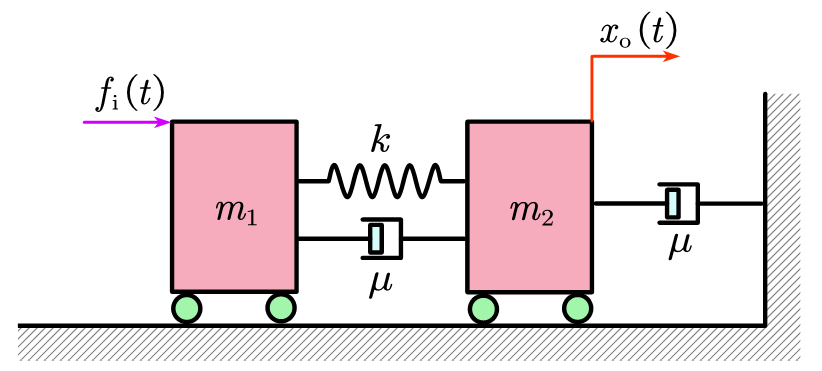
\includegraphics[width=0.6\linewidth]{T1.png}
    \caption{第一题图}
    \label{fig:T1}
\end{figure}

\subsection*{第二题（15分）}

\begin{enumerate}
    \item 某单位负反馈系统的开环传递函数为 $G(s)=\dfrac{1}{s(s+1)}$，求系统阶跃响应的上升时间 $t_\text{r}$、峰值时间 $t_\text{p}$、调整时间 $t_\text{s}$（按误差 5\% 计算）和超调量 $M_\text{p}$.
    \item 若该系统的开环传递函数为 $G(s)=\dfrac{K}{s(s+1)}$，分析 $K$ 对系统阶跃响应的动态性能的影响.
\end{enumerate}

\subsection*{第三题（15分）}

某单位反馈系统的开环传递函数为
\[
G(s)=\frac{100(s+1)}{s^2(s+10)(Ts+1)}
\]
其中 $0<T<0.1$.

\begin{enumerate}
    \item 求系统的开环放大倍数和各环节的转折频率.
    \item 画出对数幅频图（以渐近线表示），并求转折频率 $\wc$.
    \item 求系统的相角裕量 $\gamma$ 关于 $T$ 的表达式，并求系统闭环稳定时 $T$ 的最大值.
\end{enumerate}

\subsection*{第四题（15分）}

某单位负反馈系统的开环传递函数为
\[
G(s)=\frac{K}{s(s+1)(s+2)}
\]
其中 $K>0$. 画出开环传递函数的 Nyquist 图（奈奎斯特图），并根据 $K$ 的取值讨论系统的闭环稳定性.

\subsection*{第五题（15分）}

某系统的方块图如下所示. 已知 $r(t)=2\cdot1(t)$，$p(t)=1\cdot1(t)$，$d(t)=0.5\cdot1(t)$. 系统误差定义为 $e(t)=r(t)-y(t)$.

\begin{enumerate}
    \item 用 Routh 判据（劳斯判据）求系统稳定时 $K$ 的取值范围.
    \item 当 $K=3$ 时，求系统的稳态误差.
\end{enumerate}

\begin{figure}[H]
    \centering
    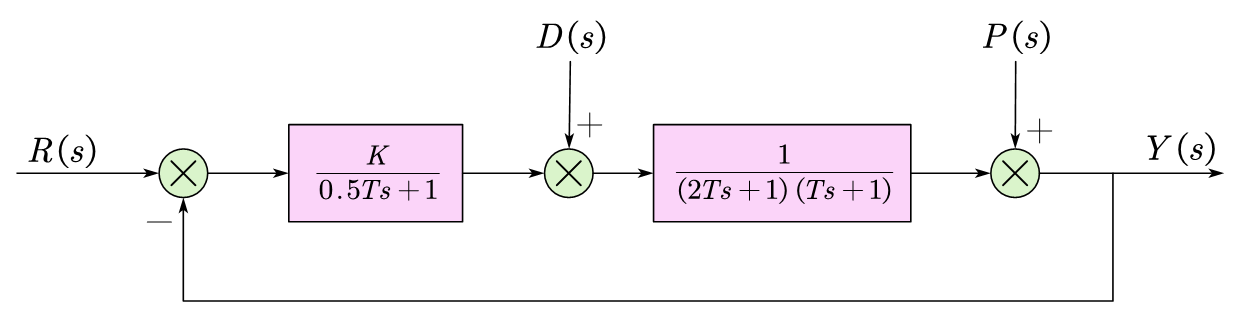
\includegraphics[width=\linewidth]{T5.png}
    \caption{第五题图}
    \label{fig:T5}
\end{figure}

\subsection*{第六题（15分）}

某单位负反馈系统的开环传递函数为
\[
G_0(s)=\frac{500}{s(0.008s+1)(0.001s+1)}
\]


\begin{enumerate}
    \item 请设计滞后校正环节，使系统性能满足如下指标：
    
    速度误差系数 $K_\text{v}\ge500\text{ s}^{-1}$，剪切频率 $\wc\approx45\rs$，相角裕量 $\gamma\ge45^\circ$.
    \item 校正后，求系统的中频宽 $h$，并求系统
    高阶最优模型的近似表达式.
\end{enumerate}

\subsection*{第七题（10分）}

某单位负反馈系统的开环传递函数为
\[
G(s)=\frac{K}{s(0.05s^2+0.4s+1)}
\]
作 $K$ 从 $0\rightarrow\infty$ 变化时的闭环根轨迹图（请写出详细过程）.

\end{document}
